\subsection{Transformer-based Neural Networks}
\citet{girdhar2019video} first incorporated the Transformer architecture into deep-learning-based action recognition tasks and proposed the Video Action Transformer network to identify and locate human actions in video data sets.
The architecture of the proposed Video Action Transformer is shown in Figure \ref{fig:ext-vatn} that the state-of-the-art model of 2019, Inflated Two-Stream 3D ConvNets (I3D) is used to extract features from video clips.
The target task of this model is to recognise and locate human actions.
It not only needs to detect the position of all people in the video but also classify the actions of each people, so the network structure is very complicated and cannot be applied on mobile devices.

\begin{figure}[!ht]
    \centering
    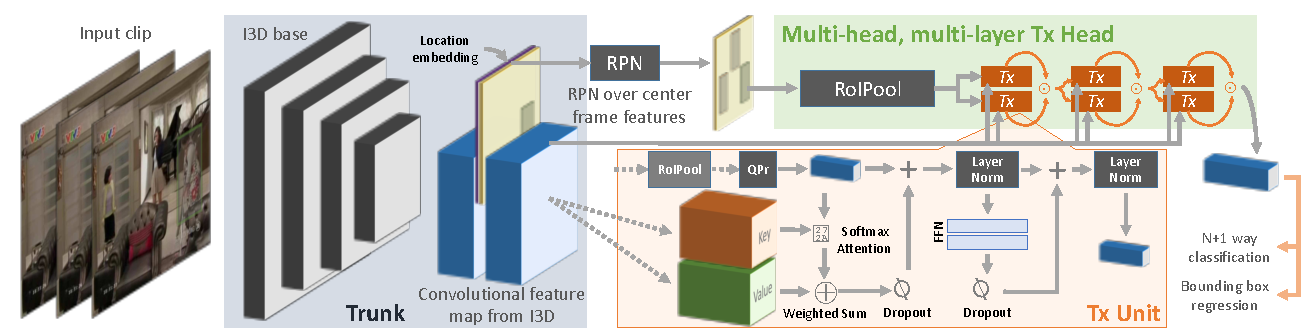
\includegraphics[width=\textwidth]{literature/imgs/ext-vatn.pdf}
    \caption{Video Action Transformer Network architecture \cite{girdhar2019video}}
    \label{fig:ext-vatn}
\end{figure}

If the target task is not to mix recognising and localising like the famous object detection model YOLO, the region proposal network (RPN) network used to obtain the position can be removed.
In this way, the paradigmatic architecture of using spatial convolution firstly and then temporal Transformer inspire research on classification tasks in the video understanding field.

In February 2021, \citet{neimark2021video} proposed the Video Transformer Network (VTN), which intuitively uses Transformer to model long-range context relationships in videos for classification tasks.
The architecture of this network is clearly shown in Figure \ref{fig:ext-vtn}.
It first uses the spatial network backbone $f(x)$ to extract features from frames, adds position embedding frame index number $PE_n$ to extracted feature vectors, and finally uses a fully connected multi-layer perceptron (MLP Head) to generate classification results.

\begin{figure}[!ht]
    \centering
    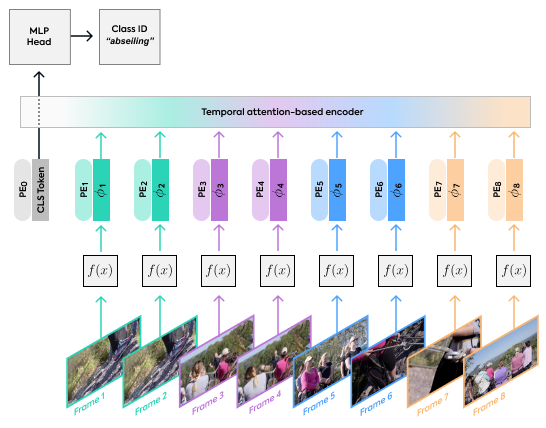
\includegraphics[width=.7\textwidth]{literature/imgs/ext-vtn.png}
    \caption{Video Transformer Network architecture \cite{neimark2021video}}
    \label{fig:ext-vtn}
\end{figure}

This research used Kinetics-400 as training and evaluation data set, and implemented the proposed model in PyTorch framework based on Facebook SlowFast\footnote{PySlowFast: video understanding codebase: \url{https://github.com/facebookresearch/SlowFast}} code base.
They used a powerful 8-V100-GPU machine for experiment, in which each GPU has 16GB memory, enabling them to conduct experiment on the large-scale video data sets.

As for contribution, they proposed a novel modular transformer-based model for the video classification task that is much more performant and efficient compared to previous methods.
Under this modular model, they also experimented and evaluated two spatial backbones, ResNet and Vision Transformer (ViT), as shown in Table \ref{tab:Video Transformer Network}.
The table shows that the ResNet (CNN-based) scheme has lower computation complicity than ViT-based scheme, which is denoted in inference GFLOP, but the ViT-based backbone brings a higher accuracy to the model.

\begin{table}[ht!]
\renewcommand{\arraystretch}{1.2}
\begin{tabularx}{\textwidth}{l|X|X|X|X|X|c}
Model & training runtime (mins) & training epochs & validation runtime (mins) & params (M) & inference GFLOPs & top-1 \\ \hline
R50-VTN & 62 & 40 & 32 & 168 & 1,059 & 71.2 \\
R101-VTN & 110 & 40 & 32 & 187 & 1,989 & 72.1 \\ \hline
ViT-B-VTN(1 layer) & 107 & 25 & 48 & 96 & 4,214 & 78.6\\
ViT-B-VTN(3 layers) & 130 & 25 & 52 & 114 & 4,218 & 78.6 
\end{tabularx}
\caption{Video Transformer Network experiment results \cite{neimark2021video}}
\label{tab:Video Transformer Network}
\end{table}

Almost at the same time in March 2021, Google researchers \citet{arnab2021vivit} published Video Vision Transformer (ViViT) that is a pure-transformer based model for video classification tasks.
The first 
Figure \ref{fig:ext-vivit} shows the architecture of the proposed model without factorisation with three model variants that factorise the different components of the transformer encoder in spatial and temporal dimensions to enhance efficiency.

\begin{figure}[!ht]
    \centering
    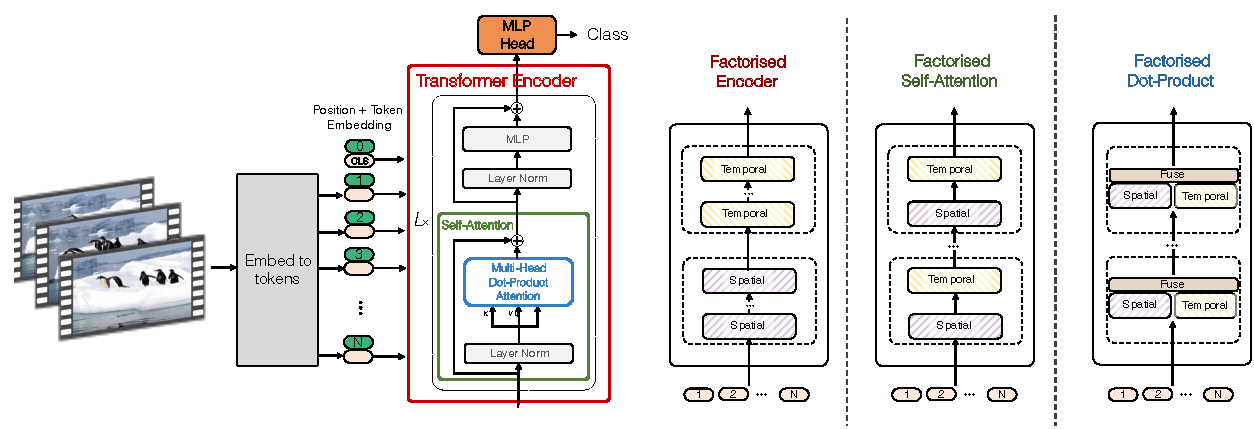
\includegraphics[width=\textwidth]{literature/imgs/ext-vivit.pdf}
    \caption{Video Vision Transformer model and factorised variants \cite{arnab2021vivit}}
    \label{fig:ext-vivit}
\end{figure}

These researches on Transformer-based networks on video classification are important references to my research.
From here on, reviewing a variety of related studies has taught me a lot and give me a clear direction for designing optimised model for the application of exam invigilation.
I need to complete the following tasks for model design in the next design stage: To design the model with appropriate spatial backbone and temporal Transformer backbone; and to optimise the model so that it can run on mobile devices with limited computing power.
